\documentclass[a4paper, 12pt]{article}
\usepackage{comment} 
\usepackage{fullpage}
\usepackage[hidelinks]{hyperref}
\usepackage{amsmath}
\usepackage{environ}
\usepackage{tabto,enumitem}
\usepackage{graphicx}

\begin{document}
\noindent
\large\textbf{SOEN 6011} \hfill \textbf{Aniket Tailor}\\
\large\textbf{Software Engineering Processes} \hfill \textbf{40195068} \\
Function 8 : Standard Deviation $\sigma$ \hfill Date: 5 August 2022\\
\normalsize Problem 1 \\

\section{Introduction}
The Standard Deviation is a measure of how spread out numbers are around the mean. It is denoted by Greek letter sigma $\sigma$. A low standard deviation implies that the data are grouped around the mean, whereas a large standard deviation shows that the data are more dispersed. In contrast, a high or low standard deviation indicates that the data points are, respectively, above or below the mean. A standard deviation that is close to zero implies that the data points are close to the mean.\\
\begin{equation*}
   (Standard Deviation) \quad \sigma = \sqrt\frac{{\Sigma (x- \overline{x})^2}}{n}
  \end{equation*}
  
Where:
    \begin{itemize}
        $\sigma$ = Standard Deviation\\
        $n$ = Size of the population\\
        $x$ = each value from population \\
        $\bar{x}$ = Mean of the population\\
    \end{itemize}

\section{Domain and Co-Domain}
\textbf{Domain:} Domain are the values which are given as input to the function. Hence in this case data values with natural and real numbers till infinity can be considered as domain.\\\\
\textbf{Co-Domain:} Co-Domain are the value which are given as output by the function. Therefore real numbers which are non negative and excluding imaginary numbers comes under Co-Domain. 

\section{Characteristics of Standard Deviation}
    \begin{itemize}[noitemsep]
        \item Only the spread or dispersion around a data set's mean is measured using the standard deviation.
        \item It can never be negative.
        \item The standard deviation is zero when all of the values in a data collection are the same because each value is equal to the mean.
        \item The higher the spread, the higher the standard deviation is for data with about the same mean.
        \item It is sensitive to outliers.
    \end{itemize}

\section{Context of Use Model}
\begin{figure}[h]
    \centering
    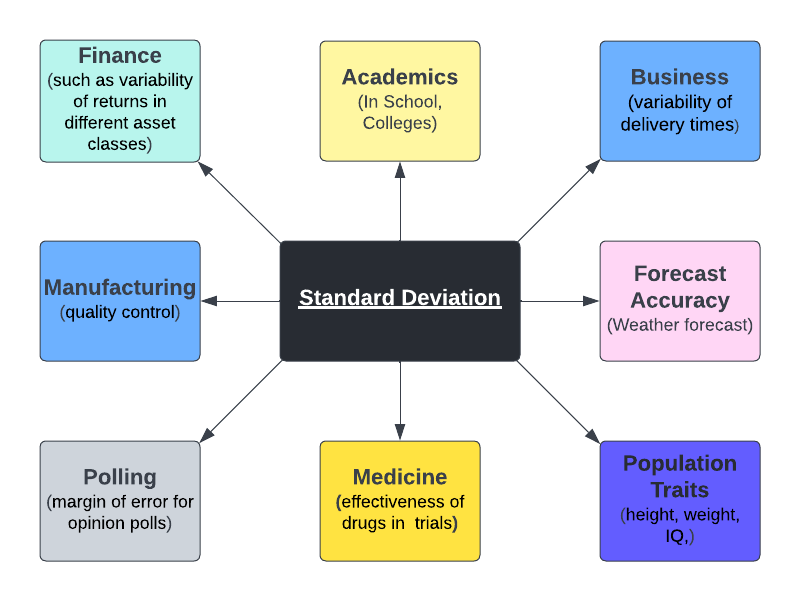
\includegraphics{Images/Context-of-use.png}
    \caption{Context of use model}
    \label{fig:Context of use model image}
\end{figure}

\newpage
\begin{thebibliography}{15}

\addcontentsline{toc}{chapter}{Bibliography}
\bibitem{1}
\href{https://en.wikipedia.org/wiki/Standard_deviation}{https://en.wikipedia.org/wiki/Standard\_deviation}

\bibitem{2}
\href{https://www.investopedia.com/terms/s/standarddeviation.asp}{https://www.investopedia.com/terms/s/standarddeviation.asp}

\bibitem{3}
\href{https://www.nlm.nih.gov/nichsr/stats\_tutorial/section2/mod8\_sd.html}{https://www.nlm.nih.gov/nichsr/stats\_tutorial/section2/mod8\_sd.html}

\end{thebibliography}
\end{document}
